\section{Contexte du Projet}
Le projet s'inscrit dans le cadre du cours Système d'information urbanisé et SOA.
L'objet du projet est de concevoir une application et l'architecture du poste de travail d'un agent commercial travaillant dans une banque. \\
Le cas étudié porte précisément sur "la gestion des contacts commerciaux" d'une banque, l'application devra donc aider le commercial dans ces tâches comme :
\begin{itemize}
\item[•]identifier et définir les contacts qu'ils doivent avoir avec leurs clients,
\item[•]permettre au chef d'agence de les répartir entre ses collaborateurs et des les réaffecter en fonction de leur disponibilité,
\item[•]Prendre rendez-vous et tenir leur agendas,
\item[•]préparer ces rendez-vous et les projets de proposition en fonction de la connaissance des clients,
\item[•]conduire les entretiens lors des rendez-vous et déclarer les résultats obtenus,
\item[•]suivre la réalisation des contacts programmés.
\end{itemize}  

\section{Risques}
Les risques majeures du projet résident dans l'organisation de l'équipe: 
\begin{itemize}
\item[•]Mauvaise répartition des tâches.
\item[•]Retard sur le planning : attente longue pour la validation des tâches par le corps enseignant.
\item[•]Absence d'un membre du groupe.
\item[•]Problème avec l'utilisation d'outil.
\end{itemize}
\section{Organisation de l'équipe}
L'équipe projet sera organisé ainsi :
\subsection{Chef de projet : Elisa \textsc{Abidh}}

Son rôle sera :
\begin{itemize}
    \item Suivi stratégique du projet
        \subitem Évaluation des risques
        \subitem Respect des objectifs
        \subitem Respects des délais
    \item Pilotage opérationnel
        \subitem Planification des taches
        \subitem Suivi et encadrement des tâches
    \item Organisation humaine
        \subitem Définition des tâches de chaque membre de l'équipe
        \subitem Résolution de conflits et arbitrage
    \item Pilotage de la production
        \subitem Suivi des résultats et livrables
        \subitem Méthodes et outils
    \item Production des livrables
\end{itemize}

\subsection{Membre de l'équipe}
Les membres de l'équipe seront amené à travailler le plus souvent en binôme. En fin de séance, chaque binôme présentera aux autres membres de l'équipe le travail qu'il a effectué en séance et le chef de projet définira les tâches à finir avant la séance d'après.  

\section{Liste des tâches, charges et répartition}
\begin{figure}[H]
	\begin{center}
		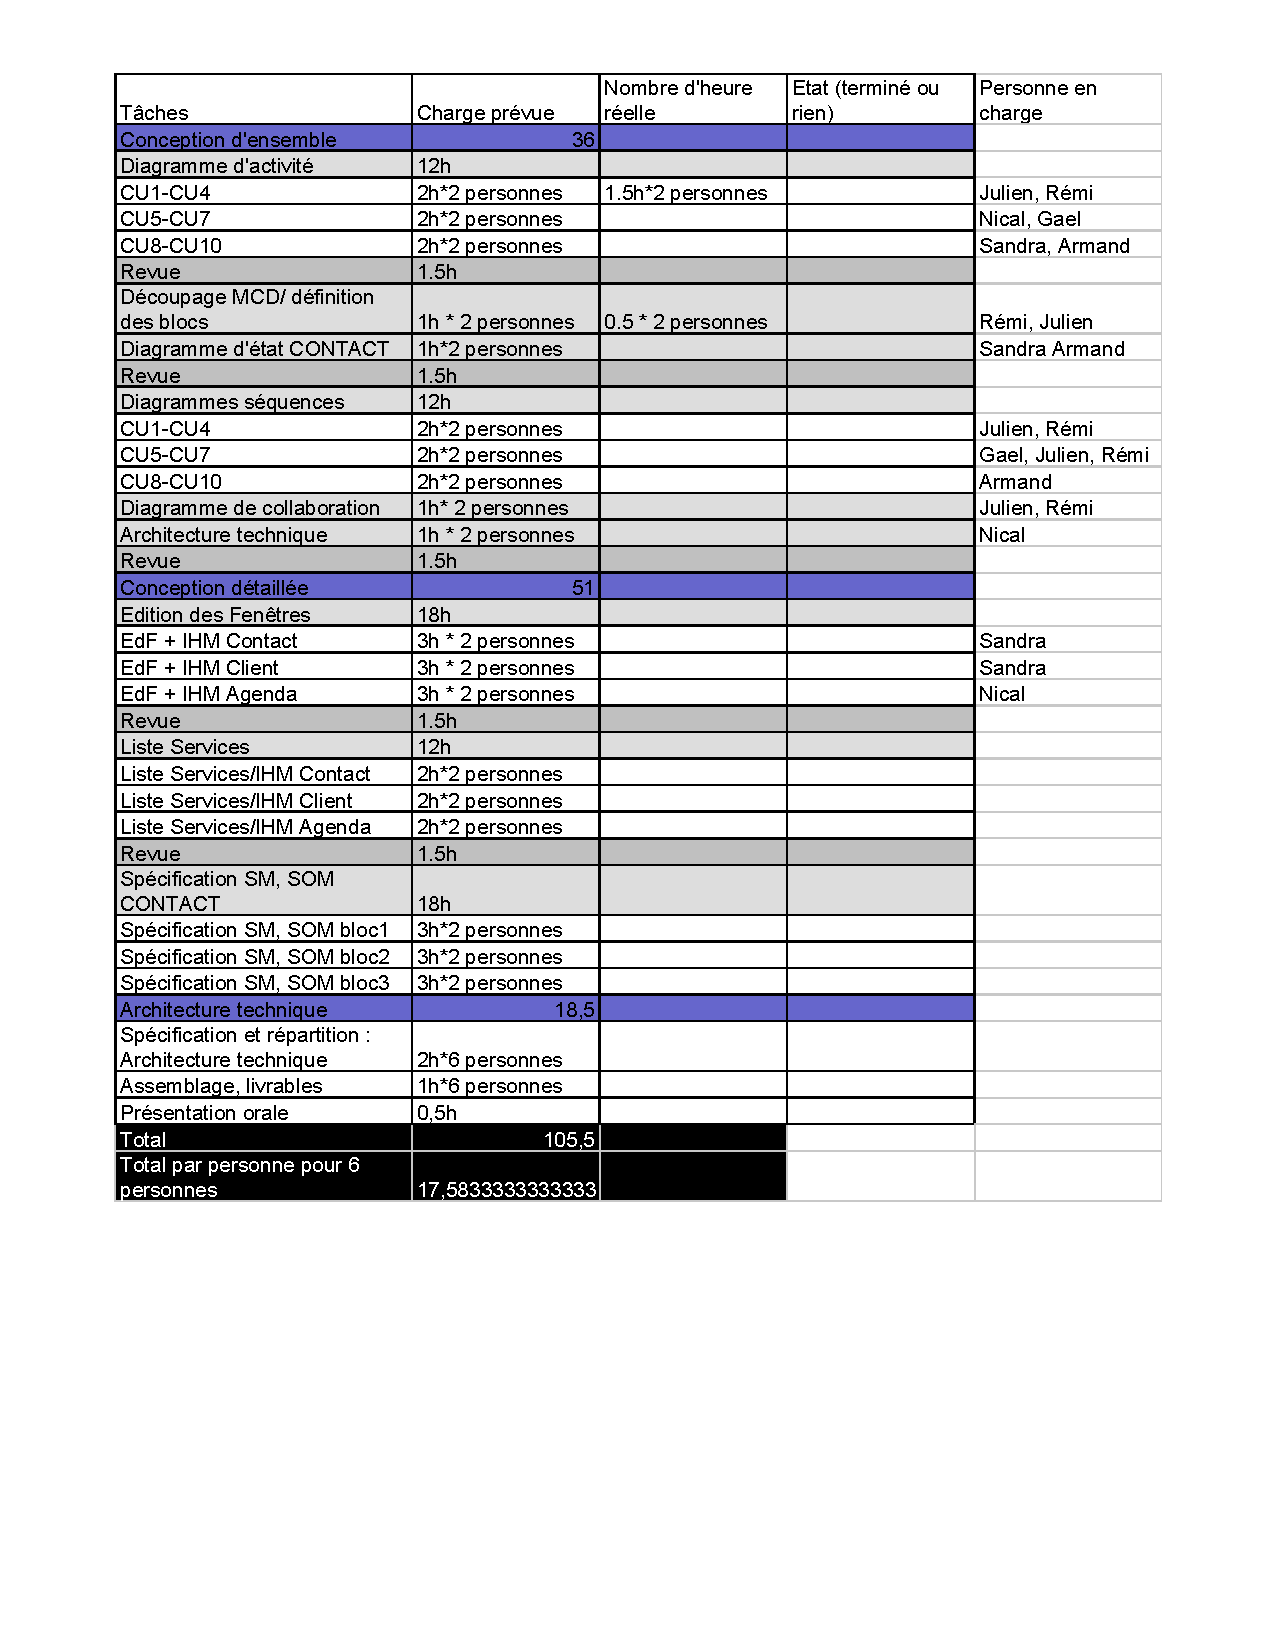
\includegraphics[scale=0.7]{SuiviTache.pdf}
		\caption{Tâches, charges}
	\end{center}
\end{figure}

Le planning permet de mettre en évidence la charge totale de travail pour chaque membre du groupe: environ 17h40 plus une heure de réunion sur l'ensemble du projet pour permettre la cohésion du groupe, ce qui fait environ 3h de travail hors séance par personne.

\section{Dépendance entre tâche}
La première dépendance est celle de respecter l'ordre des 3 grandes phases : Conception d'ensemble, conception détaillée puis Architecture technique et assemblage.\\
Au sein des 3 grandes parties nous avons les dépendances suivante : 
\begin{itemize}
\item[•]Conception d'ensemble : \\Diagrammes d'activités, Découpage MCD et définition des blocs, diagrammes de séquences et diagrammes de collaboration, architecture technique générale.

\item[•]Conception détaillée : Enchaînement des fenêtres, Liste des services, Liste des services bloc Client, spécification (SM, SOM)

\item[•]Architecture technique et assemblage :\\
Parallélisme entre Spécification, répartition et les spécifications SM, SOM.

\end{itemize}

\section{Planning prévisionnel}
\begin{itemize}
\item[•]Séance 1 : Diagramme d'activité, découpage MCD/définition des blocs, diagramme d'état.\\
Hors Séance : Finir les tâches en cours
\item[•]Séance 2 : Validation, diagramme de séquences, diagramme de collaboration, validation architecture technique et EDF + IHM.\\
Hors séance : Finir EdF + IHM
\item[•] Séance 3 : Liste des services et spécification SM,SOM.\\
Hors séance : finir les tâches en cours.
\item[•] Séance 4 : Architecture technique, assemblage, livrables et présentation orale.
Hors séance : finir la présentation orale.
\end{itemize}

\section{Livrables}
\begin{itemize}
\item[•]Document Conception d'ensemble
\item[•]Document Conception détaillée
\item[•]Document Architecture technique
\item[•]Document Bilan
\end{itemize}

\section{Outils}
\subsection{Organisation}
Pour le suivi des taches et du projet nous utilisons un google Doc. Ce document est accessible en ligne à tous moment par tous les membres de du groupe.Ils ont ainsi accès au planning prévisionnel ainsi qu'à leur fiche de suivi.\\
En ce qui concerne les livrables nous utilisons un dépôt github qui permet de faire du travail collaboratif. 
\subsection{Rédaction des livrables}
Pour la rédaction des livrables nous utilisons latex pour les contre-rendus et pour les diagrammes un logiciel en ligne : cacoo qui permet de faire des diagrammes UML. 


